\documentclass[onecolumn, draftclsnofoot,10pt, compsoc]{IEEEtran}
\usepackage{graphicx}
\usepackage{url}
\usepackage{setspace}
\usepackage[usenames,dvipsnames,svgnames,table]{xcolor}
%\usepackage{lipsum}
\usepackage[parfill]{parskip}
\parindent=0pt

\usepackage{geometry}
\geometry{textheight=9.5in, textwidth=7in}

% 1. Fill in these details
\def \CapstoneTeamName{		GROUP65}
\def \CapstoneTeamNumber{		65}
\def \GroupMemberOne{			Jacob Geddings}
\def \GroupMemberTwo{			Inhyuk Lee}
\def \GroupMemberThree{			Juan Mugica}
\def \CapstoneProjectName{		CDK Data Stream AI}
\def \CapstoneSponsorCompany{	CDK Global}
\def \CapstoneSponsorPerson{		Chris Smith}

% 2. Uncomment the appropriate line below so that the document type works
\def \DocType{		%Problem Statement
				Requirements Document
				%Technology Review
				%Design Document
				%Progress Report
				}
			
\newcommand{\NameSigPair}[1]{\par
\makebox[2.75in][r]{#1} \hfil 	\makebox[3.25in]{\makebox[2.25in]{\hrulefill} \hfill		\makebox[.75in]{\hrulefill}}
\par\vspace{-12pt} \textit{\tiny\noindent
\makebox[2.75in]{} \hfil		\makebox[3.25in]{\makebox[2.25in][r]{Signature} \hfill	\makebox[.75in][r]{Date}}}}
% 3. If the document is not to be signed, uncomment the RENEWcommand below
%\renewcommand{\NameSigPair}[1]{#1}

%%%%%%%%%%%%%%%%%%%%%%%%%%%%%%%%%%%%%%%
\begin{document}
\begin{titlepage}
    \pagenumbering{gobble}
    \begin{singlespace}
    	
\includegraphics[height=4cm]{coe_v_spot1}
        \hfill 
        % 4. If you have a logo, use this includegraphics command to put it on the coversheet.
        %\includegraphics[height=4cm]{CompanyLogo}   
        \par\vspace{.2in}
        \centering
        \scshape{
            \huge CS Capstone \DocType \par
            {\large\today}\par
            \vspace{.5in}
            \textbf{\Huge\CapstoneProjectName}\par
            \vfill
            {\large Prepared for}\par
            \Huge \CapstoneSponsorCompany\par
            \vspace{5pt}
            {\Large\CapstoneSponsorPerson\par}
            {\large Prepared by }\par
            Group\CapstoneTeamNumber\par
            % 5. comment out the line below this one if you do not wish to name your team
            %\CapstoneTeamName\par 
            \vspace{5pt}
            {\Large
                \GroupMemberOne\par
                \GroupMemberTwo\par
               \GroupMemberThree\par
            }
            \vspace{20pt}
        }
        \begin{abstract}
        % 6. Fill in your abstract    
		Our team has been assigned to assist in the development of AI for application to CDK’s existing Data Streams.
		 These streams deal mainly with the classification of documents as well as pictures and information contained within them. 
		This document outlines the various requirements our team has been tasked with fulfilling, as well constraints, time frames, platforms and strategies utilized for their completion.
		These requirements range from basic functionality pertaining to signature detection, to stretch goals such as license plate reading, car damage detection, and permit and license classification.
		
        \end{abstract}     
    \end{singlespace}
\end{titlepage}
\newpage
\pagenumbering{arabic}
\tableofcontents
% 7. uncomment this (if applicable). Consider adding a page break.
%\listoffigures
%\listoftables
\clearpage

% 8. now you write!
\section{Introduction}
Overview of SRS

\subsection{Purpose}
The purpose of this requirements document is to bring clarity to the project by indicating what the hard-line requirements are for the project to be considered a success. This will be done with the consideration that the desired end product may not be achievable and as a result will be treated as a form of research project or proof of concept.

Intended target audience for this document is our client and by extension CDK given this is their idea and the success of the project directly assists them. In addition, our instructors and teaching assistant are extensively involved in this project and they will be using this as a grading guideline. The assumption is that the reader is familiar with general concepts within computer science including artificial intelligence, common programming languages, and coding environments.


\subsection{Scope}
The product being developed will be a variant of open source AI that will be tailored to scanning submitted forms by CDK. With the inclusion of stretch goals this platform may also analyze driver licenses, vehicle imaging, or name to vehicle identification. 

This project will be capable of analyzing a submitted form to locate its signature box and check to see if it has been signed. It will also prompt the operator if it is not certain of what it is observing and if a cosigner box is also present. The format of these submissions will be in PDF format. Stretch goals include the capacity to detect expiration dates on driver’s licenses and determine what make and model of a vehicle is based on a submitted image. Additional file formats are also being considered.

Benefits from this product include reduced costs for CDK in error checking forms, rapid validation of a document, and a singular platform that can scan the various form styles that CDK possesses. Another goal of this design is the ability for it to expand upon itself and adapt to new forms that may be introduced by permitting operator confirmation or override on its assessment. 

\subsection{Definitions, Acronyms, and Abbreviations}
Open source AI is a free to access platform in which the code can be used and implemented as seen fit by the operator. OpenCV is a popular image processing example of this as well as TensorFlow and DL4j. Programming languages that may be used include C++, Python, and Java. The use of an IDE is likely, which means Integrated Development Environment which provides a more convenient setup for coding. Examples of IDE’s include Microsoft Visual Studio and Eclipse. Black box design means that the user does not need to understand the internal functions of the program, just what it wants as input and what the user will receive as the output. 

\subsection{References}
[1] IEEE Software Engineering Standards Committee, “IEEE Std 830-1998, IEEE Recommended Practice for Software Requirements Specifications”, June 25, 1998.

\subsection{Overview}
The remainder of the requirements document will contain a greater look into what precisely the project entails. This is going to involve looking at where the project stands for CDK and how it will be utilized as well as the products functions and characteristics for a user. Mention will also be made towards potential constraints placed upon the program.

The following section will be a general overview and description of the project, primary focus being placed on functions, characteristics, constraints, and assumptions/dependencies. After that there will be a section on specific requirements that will bring mention to potential interfacing concerns as well as performance metrics and standards compliance. The document is designed to follow the IEEE Software Engineering Standards [1].


\section{Overall Description}
\subsection{Product Perspective}
The core objective as well as the stretch goals all conclude that this product will be an independent platform. For this project, we will explore the potential of A.I. and create the foundation of CDK’s own AI platform.

The signature detection and drivers license verification software must support various personal computers such as desktop, laptop, and tablet as an input source. This software will first receive a PDF file of a document as its input. It will then compute the data and give result or feedback to user. With that in mind, the software needs to be robust enough to compute large set of data. Similarly, within our stretch goals, vehicle model detection software must also support various personal computers and be robust enough to evaluate large data. However, it must also support portable devices with camera such as phone and tablet. Software should first take photo from camera then it evaluates the photo and returns model number.

\subsection{Product Functions}
Main goal
The function of this software is detecting the location of the signature box and determine whether it is signed or unsigned. If document is unsigned: software must provide information of location and quantity of missing components. Also, the program must be capable of making a reasonable guess on whether a signature is sufficiently binding. This entails the AI must be capable of distinguishing between a simple mark in the signature window and an actual signature.

Stretch goal
License validation software: This software must validate whether given photo is driver’s license or not. First, it must validate the format of driver’s license and check legal information such as expiration date.

Vehicle model detection software: Vehicle model detection software must be able to determine the specific model number from appearance of the vehicle. Software will first take photos or video of vehicle taken from different angle. It will determine vehicle model by narrowing down the information. For example, software will search sequentially for make, model, and year.

\subsection{User Characteristics}
The intended user of the software is vehicle retailers. We can assume a low degree of understanding on artificial intelligence. Therefore, software must be designed as black box model. To accompany this structure the user interface must be agreeable for them. Lastly, the program must not overburden the operator, it will take a single file as input to scan and return a conclusion to the user.


\subsection{Constraints}
There are few constraints on CDK A.I. data stream project. First, software must be standalone. The future goal of this project is to build CDK’s own platform, so software must be independent. In addition, project must be kept in open source. The software must be made in such a way that, once our team has completed its work, the project be taken over by a new team within CDK. To meet this demand the need for thorough documentation of implementation is vital. This project will also have limits on testing due to the privacy issue surrounding actual consumer data. Since the data that signature detecting and license validation software compute contains personal data, testing data must be done on dummy documents and licenses. The last constraint is that product must function on its own without the additional use or maintenance of outside software. Since the users of the product are unlikely to be familiar with the internal workings the interface for them must sufficiently mask the technical workings of the program only provide a clean and simple menu.

\subsection{Assumptions and Dependencies}

All images provided by the client are sanitized and free of legal conflicts. Cloud based deployment services will be provided by the client. From a developing and testing standpoint, this project will be developped in C++ utilizing the OpenCV picture formatting library. This library assumes that the system is running GCC 4.4.x or later as well as CMake 2.8.7 or higher. 



\section{Specific Requirements}

\subsection{External Interface Requirements}
The main interface design principle of this software are intuitiveness and simplicity. Since potential users of the software are people who knows little or non about machine intelligence, software must be easy to use without knowing any of the background information.

\subsubsection{User Interfaces}
The signature detection software interface window is consist with four sections which are top menu bar, pop-up window, detection window, and feedback window. $\langle$Figure 1$\rangle$ shows the interface structure of signature detection software.

Following are descriptions of each section:

\begin{description}
	\item[1.]Top Menu Bar:  There are five buttons that serve different functions for this section. Starting from the left side: load file, save progress, start detection, stop detection, and continue detection. 'Load File' button loads up the file that needs to be processed. 'Save Progress' button allow user to save the progress of currently active work and start it later. When a user presses either load or save it will display a pop-up window for each respectively as shown in $\langle$Figure 2$\rangle$. Detection buttons allow user to start, stop, and continue the detection.

	\item[2.]Pop-up Window: Whenever an error is detected or load/save file button is pressed. This window will show at the middle of the screen to either alert of an error or indicate a sub window that gives proper interaction control.

	\item[3.]Detection Window: This window displays current working document. Software scan through the given document to find signature box. Orange box on $\langle$Figure 1$\rangle$ denotes where the software is currently looking at, so user can get a sense of how much work is done. It also highlights the location of missing or incorrect signatures with a red box $\langle$Figure 1$\rangle$. This box will be shown whenever software locates missing or incorrect signatures.

	\item[4.]Information Window: Will show more detailed information about each active document. It displays important information such as the number of missing signature, the number of incorrect signatures, presence of co-sign box, the number of pages finished detection, and the number of pages on the queue.

\end{description}

\begin{figure}[h]
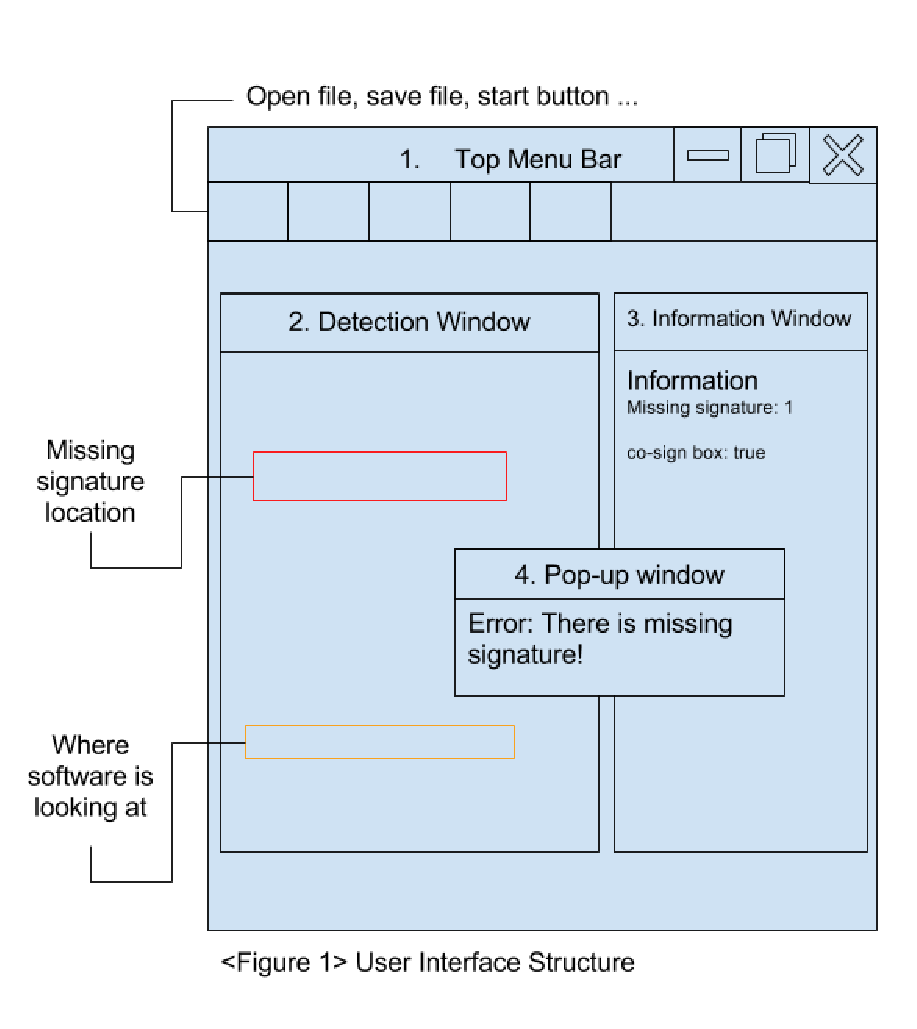
\includegraphics[width= 7.5cm]{Figure_1}
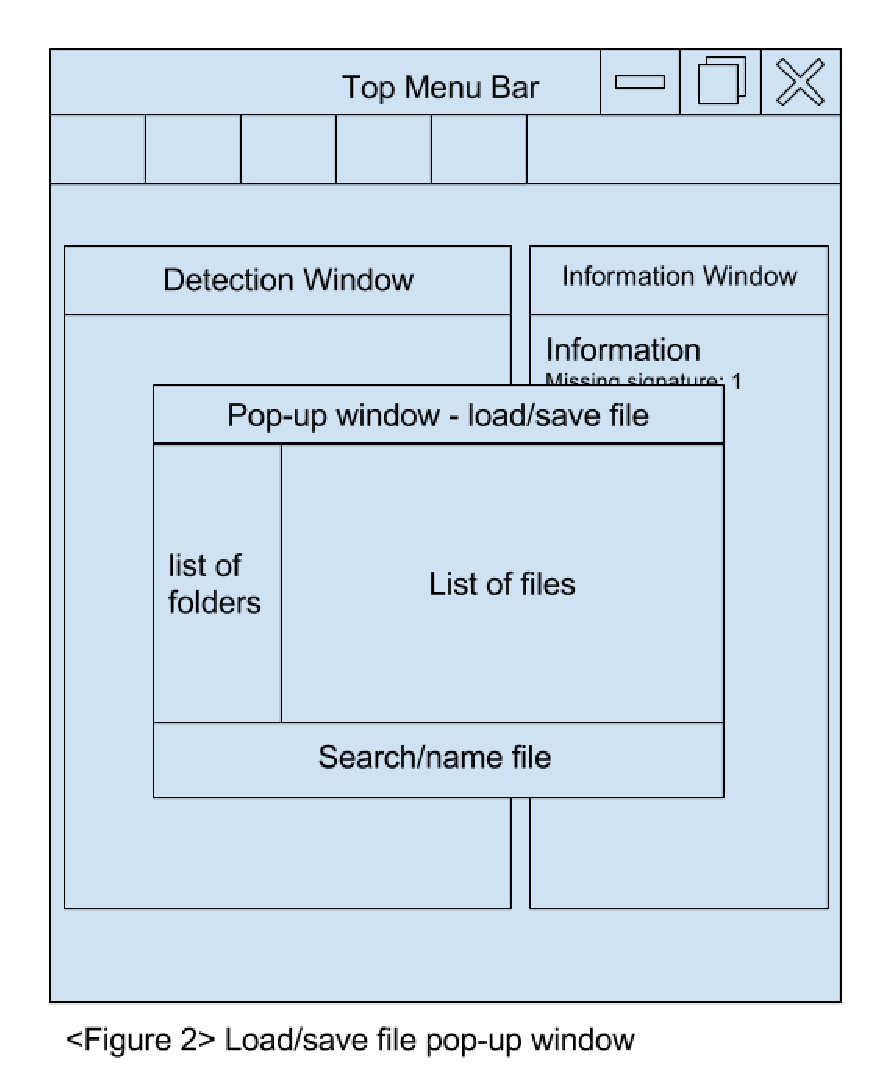
\includegraphics[width= 7.5cm]{Figure_2}
\centering
\end{figure}

\subsubsection{Hardware interfaces}
This project does not include building any specific hardware. Therefore, there is no hardware interface for this software.

\subsubsection{Software interfaces}
The software will be built utilizing a Linux installation of the OpenCV image processing framework. In order to ensure the program is portable, the project will utilize the Docker container software. Cloud deployment will be handled by the Amazon Web Services platform.

\subsubsection{Communications interfaces}
For this project, all software acts independently. In the future, the project will be developed to communicate with other instances of itself in order to improve its performance.  However, in this project, building the individual first instance is the main focus.


\subsection{System Features}
\subsubsection{Signature detecting capability}\vspace{.5cm}

\hfill\begin{minipage}{\dimexpr\textwidth-1cm}
\paragraph{Introduction/Purpose of feature}
The program must be able to detect if a document contains a signature regardless of the documents formatting.
\paragraph{Stimulus/Response sequence}
The program will parse a PDF image of a document, or a document in PDF format, and output a percentage based estimation as to whether it contains a signature.
\paragraph{Functional Requirements}
Signature detection must be functional for all types of document formats regardless of the type so long as they are presented in PDF file format. 
\end{minipage}
\vspace{.75cm}


\subsubsection{Missing signature detection}\vspace{.5cm}

\hfill\begin{minipage}{\dimexpr\textwidth-1cm}
\paragraph{Introduction/Purpose of feature}
The program must be able to detect if a document contains a space where there should be a signature regardless of the format of the form.
\paragraph{Stimulus/Response sequence}
The program will parse a PDF image of a document , or a document in PDF format, and output a percentage based estimation as to whether it contains a space where a signature is missing.
\paragraph{Functional Requirements}
Signature detection must be functional for all types of document formats regardless of the type so long as they are presented in PDF file format. 
\end{minipage}
\vspace{.75cm}

\subsubsection{Multiple signature and multiple missing signature capability}\vspace{.5cm}

\hfill\begin{minipage}{\dimexpr\textwidth-2cm}
\paragraph{Introduction/Purpose of feature}
The program must be able to perform feature 3.2.1 for every signature contained within the document. The program must also be able to perform feature 3.2.2 for every space that is missing a signature within the document
\paragraph{Stimulus/Response sequence}
The program will parse a PDF image of a document, or a document in PDF format, and output percent estimates for features 3.2.1 and 3.2.2 at every instance deemed applicable. 
\paragraph{Functional Requirements}
Multiple signature and multiple missing signature capabilities must be functional for all types of document formats regardless of the type so long as they are presented in PDF file format.
\end{minipage}

\vspace{.75cm}
\textbf{\textit{The following features are part of the groups stretch goals and are to be completed once the aforementioned features work to the satisfaction of the client. 
}}
\vspace{.75cm}


\subsubsection{Car detection within image}\vspace{.5cm}

\hfill\begin{minipage}{\dimexpr\textwidth-1cm}
\paragraph{Introduction/Purpose of feature}
The program must detect if a given picture contains a car within it.
\paragraph{Stimulus/Response sequence}
The program will parse a PDF image and output a percentage based estimate as to whether it contains a car.
\paragraph{Functional Requirements}
The program must be able to detect cars within any picture presented in PDF format.
\end{minipage}
\vspace{.75cm}

\subsubsection{License and Permit detection within document}\vspace{.5cm}

\hfill\begin{minipage}{\dimexpr\textwidth-1cm}
\paragraph{Introduction/Purpose of feature}
The program must detect if a document contains a license or a permit regardless of the format of the form.
\paragraph{Stimulus/Response sequence}
The program will parse a PDF image of a document , or a document in PDF format, and output a percentage based estimation as to whether it contains a license, or a permit.
\paragraph{Functional Requirements}
The program must be able to detect permits and licenses within any document presented in PDF format.
\end{minipage}
\vspace{.75cm}

\subsubsection{Parse license plate, license, and permit text into machine readable format}\vspace{.5cm}

\hfill\begin{minipage}{\dimexpr\textwidth-1cm}
\paragraph{Introduction/Purpose of feature}
Once the program can perform features 3.2.3 and 3.2.4, it must then parse the contents of these forms into machine readable format. This will allow the user to utilize this information to validate a client’s identity, ties to the vehicle, etc.. For this task, we will utilize Google’s Vision API.
\paragraph{Stimulus/Response sequence}
The program will parse a license, permit, or license plate image in PDF format and extract the information presented into a machine readable format. 
\paragraph{Functional Requirements}
The program must be able to read information within any license plate, license, or permit regardless of the origin so long as they are presented in a PDF format.  
\end{minipage}
\vspace{.75cm}

\subsubsection{Damage recognition}\vspace{.5cm}

\hfill\begin{minipage}{\dimexpr\textwidth-1cm}
\paragraph{Introduction/Purpose of feature}
The program must be able to parse a picture of a vehicle and detect whether this vehicle has sustained damage. Often CDK employees must go through pictures of vehicles in order to assess if they have been damaged. This feature aims at discarding all vehicles with no damage lessening the amount of pictures that must be assessed for damage. 
\paragraph{Stimulus/Response sequence}
The program will parse a picture of a car in PDF format and output a percentage estimate as to whether the car has been damaged. 
\paragraph{Functional Requirements}
The program must be able to detect damage within any picture of a car so long as it is submitted in PDF format. 
\end{minipage}
\vspace{.75cm}

\subsubsection{Make and Model detection}\vspace{.5cm}

\hfill\begin{minipage}{\dimexpr\textwidth-1cm}
\paragraph{Introduction/Purpose of feature}
The program will parse the picture of a car and attempt to discern the make and the model.
\paragraph{Stimulus/Response sequence}
The program will parse an image of car in PDF format and output a number of percentages assessing what the possible make and model combination might be for the vehicle. 
\paragraph{Functional Requirements}
The program must be able to detect the make and model of a vehicle regardless of the make and model so long as the picture is of a car, and is submitted in PDF format. 
\end{minipage}
\vspace{.75cm}

\subsection{Performance requirements}
This program will utilize deep learning algorithms to achieve all features except for 3.2.5. To do so, the program must run continuously for extended periods of time in order to ensure optimal learning time frames. The program must be able to catch errors and continue running unless the error is fatal. Segmentation faults, memory depletion and hardware errors are all considered fatal, all other errors must be caught, handled, and notified to the user. 


\subsection{Design Constraints}
The program is free of design constraints so long as the interface ensures ease of access and interaction between the different components for all end users. This pertains to the ease of submission of pictures and documents to the software, as well as the presentation of all results in a readable and comprehensive manner. 


\subsection{Software system attributes}
The program will require a platform in which to run uninterrupted for extended periods of time. The platform must be accessible to ensure that modification can be made whenever deemed necessary. The platform must be portable to ensure that the software can be deployed in a wide range of environments.  Finally, the platform must be able to support heavy usage of memory resources to ensure the software does not encounter depletion of memory issues. 

\pagebreak

\section{Appendix}

This section details the groups schedule in order to complete the tasks per the school year of 2017. Included is a Gantt chart detailing what the specific task is and the time frame over which they're scheduled to take place.

Fall Term
\begin{description}
	\item[Week 6:]10/29
	\item[End:]   Friday, December 8, 2017
\end{description}


Winter term
\begin{description}
	\item[Begin:]Monday, January 8, 2018
	\item[End:]	 Friday, March 23, 2018
\end{description}


Spring Term
\begin{description}
	\item[Begin:]Monday, April 2, 2018
	\item[Expo:] 	Tentatively May 18, 2018
	\item[End:]			Friday, June 15, 2018
\end{description}


\begin{figure}[h]
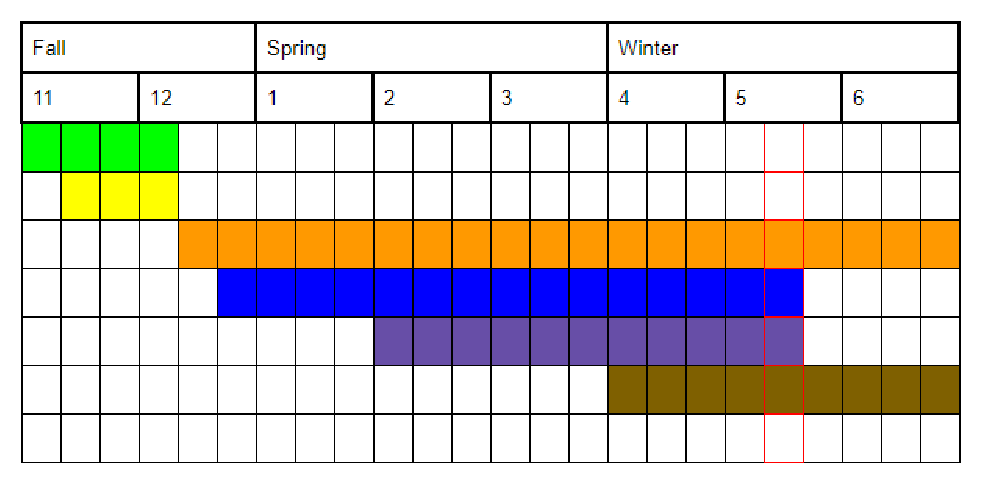
\includegraphics[height= 5cm]{Gantt}
\centering
\end{figure}

Practice
\begin{description}
	\color{green}
	\item[--]Study machine learning framework
	\color{yellow}
	\item[--]Build Small texture detecting program
\end{description}

\color{black}
Main: Build first prototype
\begin{description}
	\color{Orange}
	\item[--]Study on texture detecting A.I. algorithm
	\color{blue}
	\item[--]Build program that detects handwritten signatures from document
	\color{purple}
	\item[--]Adapt program to accept ranging document formats
	\begin{description}
		\color{black}
		\item[--]Data feeding
		\item[--]Check License information
		\item[--]Check permit information
	\end{description}
	\color{brown}
	\item[--]Optimize the program
	\begin{description}
		\color{black}
		\item[--]Debugging
	\end{description}
\end{description}
Stretch Goals (to be scheduled after completion of original goals)
\begin{description}
	\item[--]Detect the model of a vehicle
	\item[--]Detect the make of a vehicle
	\item[--]Detect/read license plate information
	\item[--]Detect/read license and permit information
	\item[--]Gather information of the condition of the vehicle (e.g.: dents, cracks and scratches)
\end{description}
\end{document}